\section{Projektorganisation}

\subsection{Auswahl der Projektstruktur}

Bevor mit der Planung des angestrebten Projekts begonnen werden kann, muss zunächst eine grundlegende Entscheidung über das Vorgehen und das Projektmanagementmethode getroffen werden. Da die verschiedenen Methoden bereits bei der Projektplanung teilweise bedeutende Unterschiede aufweisen, muss diese Entscheidung bereits vor der Planungsphase getroffen werden.

\subsection{Kurzer Vergleich gängiger Projektmanagementoptionen}
\label{subsec:pmstrukturen}

Grundsätzlich wird beim Projektmanagement zwischen drei Ansätzen unterschieden:\\

\begin{table}[ht]
    \centering
    \begin{tabularx}{\textwidth}{|l|X|X|} 
        \hline
        Klassisch & Linear Sequentiell. Erst wenn die Arbeiten eines Schrittes abgeschlossen wurden, wird mit dem nächsten begonnen. Die Abfolge und Abläufe der Schritte sind statisch und ein Abweichen vom Projektplan ist nicht ohne weiteres Möglich. Bei Projekten dieser Art wird viel Zeit auf eine sehr detailierte Vorplanung gelegt, die dann über fest definierte Meilensteine überprüft und gesteuert werden kann. Ein bekannter Vertreter dieses Ansatzes ist das Wasserfallmodell. \\
        \hline
        Agil & Inkrementell Iterativ. Während des Projektes wird das Endprodukt immer weiter verfeinert. Die Vorplanung bei Projekten dieser Art ist im Vergleich zum klassischen Vorgehen deutlich weniger detailiert. Viel mehr werden die Anforderungen in ständiger Kommunikation mit dem Kunden/Auftraggeber kontinuierlich überprüft und verfeinert, in der Regel nach dem Erreichen von Zwischenschritten (Inkrementen).  Ein bekannter Vertreter dieses Ansatzes ist Scrum. \\
        \hline
        Hybrid & Der Hybride Ansatz verbindet Elemente des Klassischen und des Agilen Projektmanagements um sich so die Vorteile beider Vorgehensweisen zu Nutze zu machen. Etwa indem die umfassende Projektstruktur klassisch aufgebaut ist um eine solide Struktur und klare Planbarkeit sicherzustellen, aber auf der Teamebene die Dynamik des 			agilen Ansatzes nutzt um bei der Erstellung des eigentlichen Projektprodukts flexibel agieren zu können. Eine Möglichkeit diesen Ansatz umzusetzen ist Prince2 (diese Methode bietet auch die Option rein klassisch vorzugehen)\\
        \hline
    \end{tabularx}
    \caption{Kurzübersicht Projektmanagementoptionen}
    \label{tab:pmOptionen}
\end{table}

\subsection{Agiles Vorgehen im Projekt}
\label{subsec:agilesVorgehen}

Eine etablierte Möglichkeit festzustellen, welches Vorgehen sich für ein konkretes Projekt eignet ist die Stacey Matrix.\\

\begin{figure}[!h]
\centering
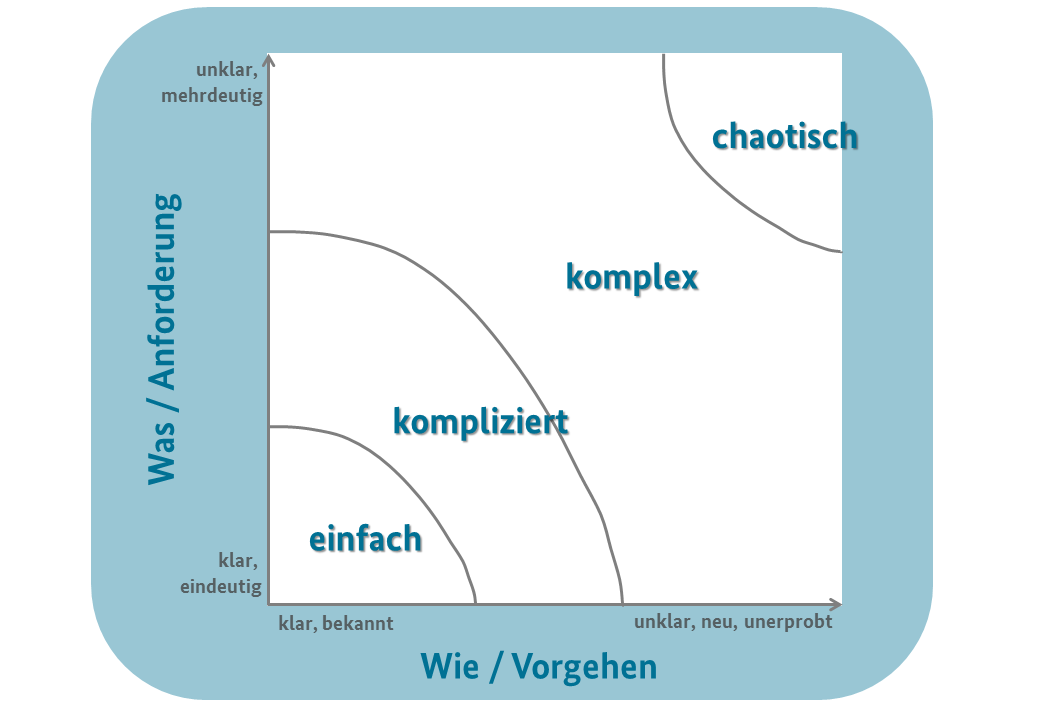
\includegraphics[width=6.24cm, height=4.32cm]{StaceyMatrix}
\caption{Stacey Matrix (\url{https://www.bva.bund.de/DE/Services/Behoerden/Beratung/Beratungszentrum/GrossPM/Wissenspool/_documents/Standardartikel/stda-stacey-matrix.html})}
\end{figure}

Im Bezug auf das geplante Projekt sind die Anforderungen noch nicht wirklich klar ausformuliert. Die Geschäftsführung hat eine Vision, eine grobe Idee und keinen klaren Katalog an sorgfältig definierten Anforderungen. Die Anforderungen sind also unklar.\\

Das Vorgehen an sich ist innerhalb des organisatorischen Ökosystems der Philetairus Immobilien GmbH unklar und unerprobt. Die IT Abteilung hat zuvor noch keine größeren Entwicklungsprojekte durchgeführt, daher ist auf diesem Gebiet wenig Erfahrung vorhanden und die Einbindung und  Einarbeitung der neuen Mitarbeiter kommt noch hinzu. Es gibt keine Erfahrungswerte innerhalb des Unternehmens auf die zurückgegriffen werden könnte, das Vorgehen ist daher unklar und unerprobt.\\

Basierend auf diesen Parametern ist dieses Projekt als Komplex einzuschätzen, daher ist ein agiles Vorgehen ratsam um der bestehenden Unklarheit möglichst flexibel zu begegnen und während des Projektes die geeigneten Methoden und Techniken zu erarbeiten. Für ein klassisches Vorgehen wäre eine langwierige Vorbereitungsphase notwendig, in der die genauen Anforderungen ermittelt werden müssten, bevor das Projekt überhaupt starten könnte.\\

Ein weiterer Vorteil des agilen Vorgehens in diesem Fall besteht in der zuvor beschriebenen Iterativen und Inkrementellen Vorgehensweise. So kann in regelmäßigen Abständen der Fortschritt überprüft werden und gegebenenfalls Anpassungen und Ergänzungen an den Anforderungen vorgenommen werden. Prinzipiell wäre das auch bei einem traditionellen Ansatz möglich, allerdings ist es dort mit einem größeren Aufwand verbunden einmal fixierte Projektanforderungen zu ändern .\\

Diese Flexibilität steht in direktem Zusammenhang mit der engen Einbindung der (in diesem Fall unternehmensinternen) Auftraggeber, die typisch für agiles Projektmanagement ist. Während die Auftraggeber bei klassischen Vorgehen konkrete Anforderungen zu Beginn des Projektes definieren und diese dann entweder zum Ende (oder zu festgelegten Meilensteinen) prüfen und abnehmen, stehen der Auftraggeber (oder dessen Vertreter) bei agilen Vorgehen in ständiger Kommunikation mit dem Entwicklerteam, prüfen die Zwischenprodukte (Inkremente) und beteiligen sich aktiv an der Anpassung und Aktualisierung der Anforderungen (zum Beispiel über das Product Backlog, siehe ~\ref{subsec:productGoalBacklog}).\\

Zu der Flexibilität des Vorgehens und des geringen Aufwands der Projektvorbereitung kommt ein weiterer Vorteil hinzu - die vergleichsweise hohe Anzahl der neuen Mitarbeiter, die durch die Erweiterung der IT Abteilung hinzugekommen sind. Diese sind noch nicht vollständig in die Unternehmensstrukturen integriert, auch hier bietet der agile Ansatz den Vorteil, da er auf flache Hierachien und Zusammenarbeit auf Augenhöhe setzt und die neuen Mitarbeiter somit schneller in das Ökosystem integriert werden können.\\

Aus diesen Gründen wurde der Entschluss gefasst, das Projekt agil anzugehen. Allerdings gab es von Seiten der Geschäftsleitungen einige Bedenken bezüglich eines rein agilen Vorgehens, weshalb weitere Überlegungen zur Projektstruktur angestellt wurden.\\
\subsection{Hybrides Vorgehen im Projekt}

Während die Stacey Matrix hilft das Projekt zu beurteilen und eine Entscheidung für klassisches oder agiles Vorgehen im Projekt zu treffen, gibt es andere Methoden und Hilfsmittel, den Projektkontext, nicht das Projekt als solches zu betrachten und einzuordnen. Eines davon ist das Agilometer:\\

\begin{figure}[hbt!]
\centering
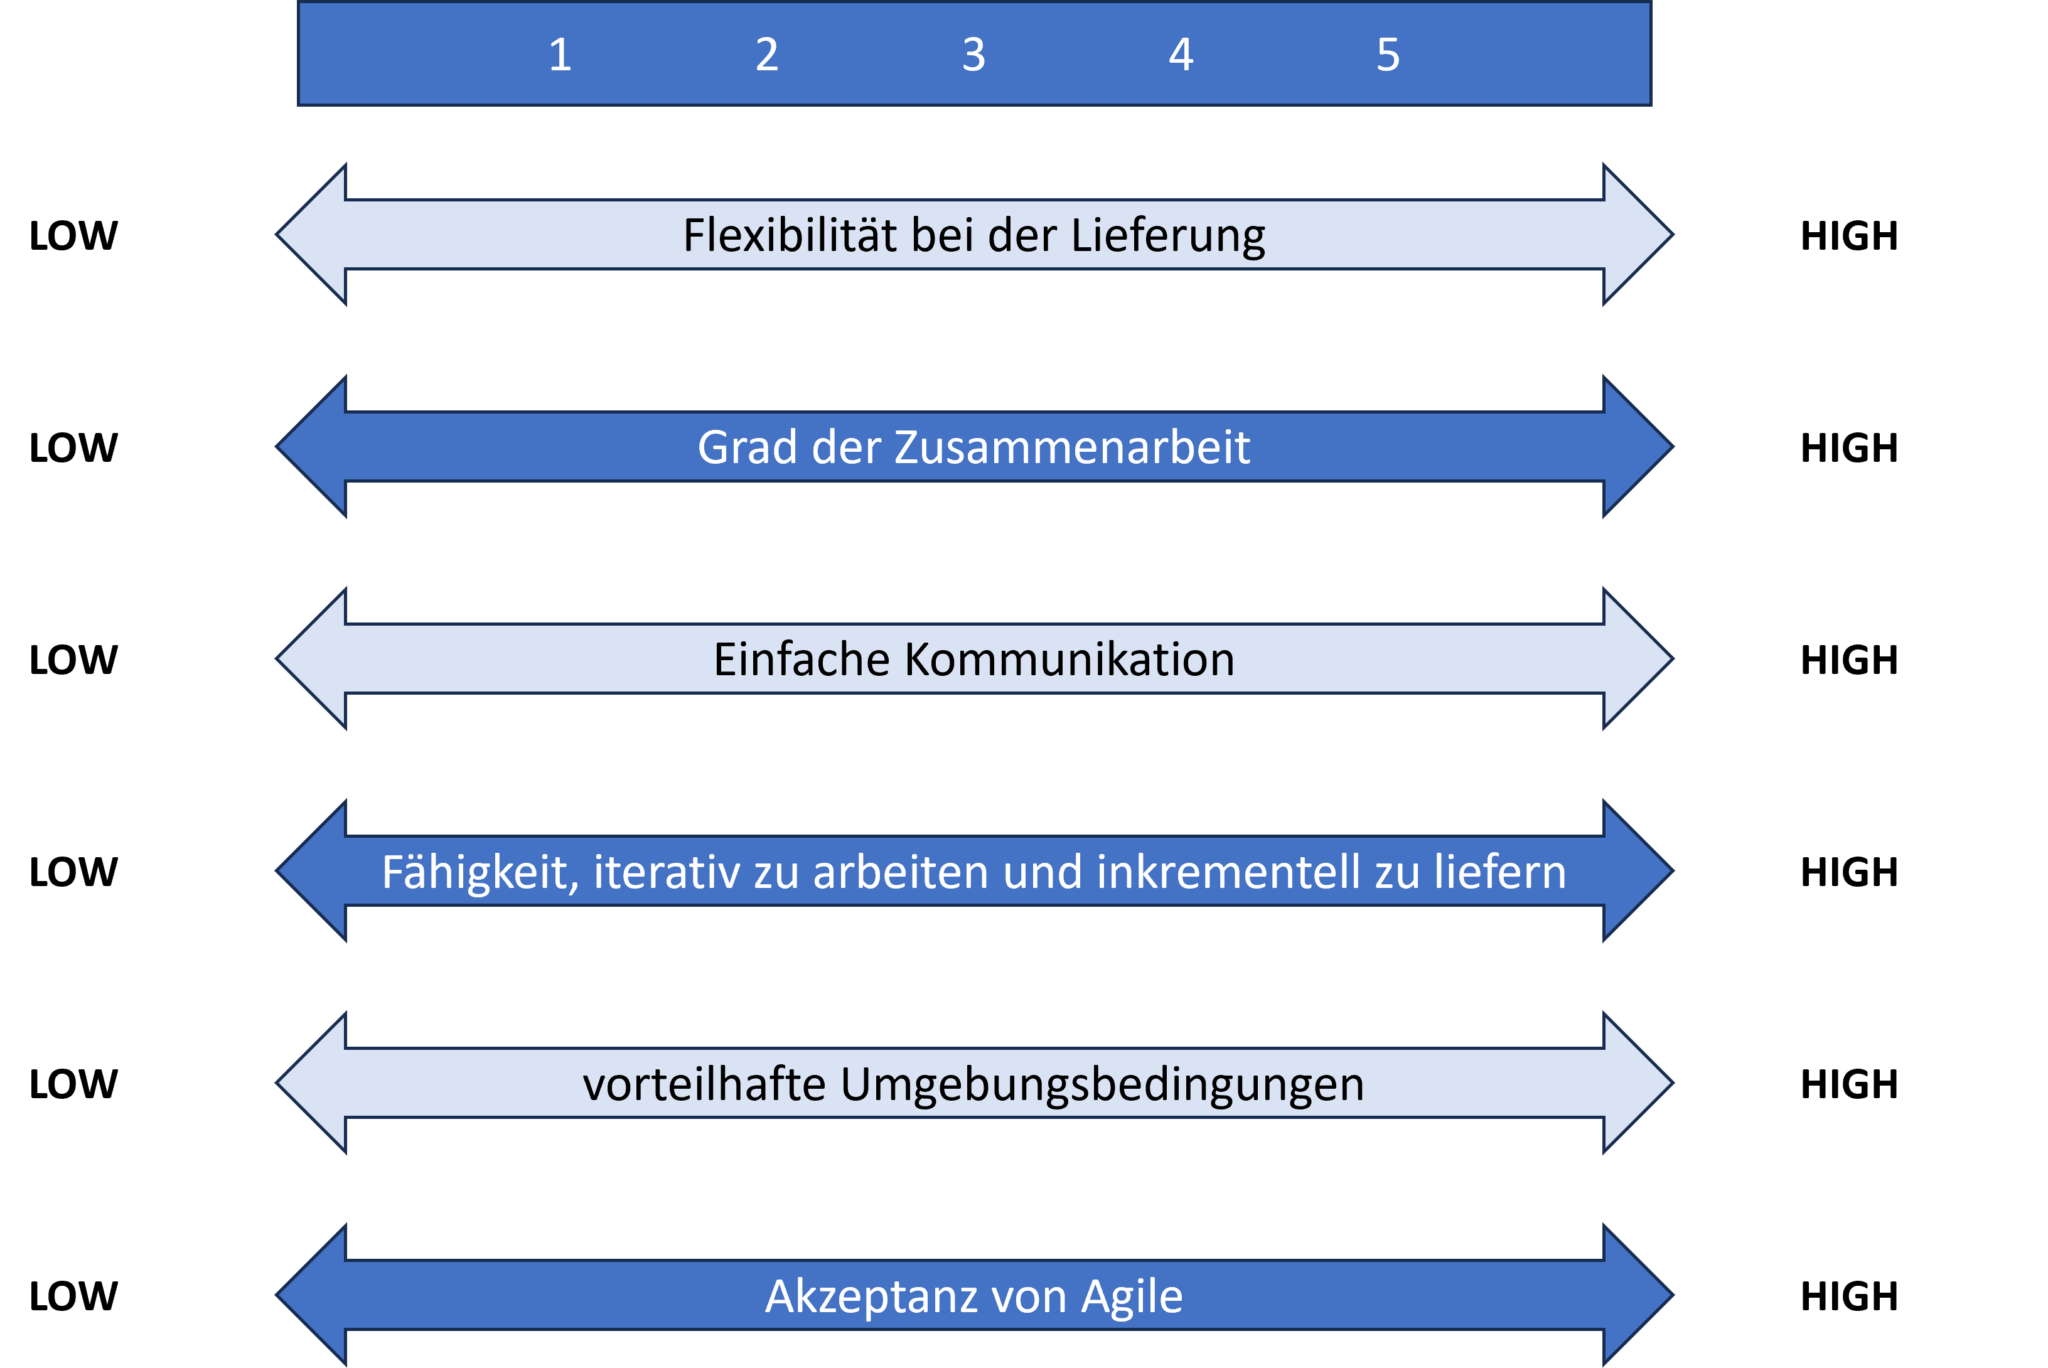
\includegraphics[width=9.69cm, height=6.48cm]{Agilometer}
\caption{Agilometer (\url{https://www.pureconsultant.de/de/agile/agilometer/})}
\end{figure}

Betrachtet man die Philetairus Immobilien GmbH, so ist der agile Reifegrad äußerst niedrig. Es gibt das Bestreben, zumindest auf der für das vorliegende Projekt relevanten Ebene agiler zu agieren, doch die mangelnde praktische Erfahrung bei der umsetzung von agilen Projekten, die immer noch bestehende Skepsis der Unternehmensführung und die große Anzahl von neuen Mitarbeitern in der ausführenden Abteilung deuten darauf hin, dass ein rein agiles Vorgehen keine sinnvolle Wahl wäre.\\

Ein klassisches Vorgehen nach dem Wasserfall- oder V-Modell wäre aufgrund der noch recht unkonkreten Zielsetzung des Projektes auch wenig praktikabel, da für diese Vorgehensweise mit Lasten- und Pflichtenheft die Anforderungen möglichst konkret und unmissverständlich formuliert werden müssen, bevor das Projekt initiiert werden kann.\\

Aus diesem Grund ist für das Vorhaben ein Hybrides Vorgehen, welches klassisches und agiles Vorgehen miteinander verbindet ideal. Für das agile Vorgehen fiel die Entscheidung auf Scrum (siehe ~\ref{subsec:agilesVorgehen}), den klassischen Rahmen soll Prince2 bilden.\\

Prince2 gibt klare Vorgaben, wie das Projektmanagementteam strukturiert sein sollte, für die Planung auf der Teamebene gibt es allerdings keine starren Richtlinien. Daher ist es möglich, ein hybrides Vorgehen zu wählen. Im Fall dieses Projekts wurde die Entscheidung für diese diese Variante getroffen: traditionelles Vorgehen auf der Entscheidungsebene und agiles Vorgehen auf der operativen Ebene. Somit bleibt ein großes Maß an Kontrolle erhalten, ohne die Vorteile des agilen Vorgehens zu sehr zu beschneiden.\\

Auf der anderen Seite definiert der Scrum Guide sehr genau die Rollen und Verantwortlichkeiten auf der Teamebene sowie das Vorgehen während der Entwicklung, die genaue Einbindung in die Unternehmensorganisation wird allerdings nicht konkret vorgegeben, somit ergänzen sich die beiden Vorgehensweisen, da es keine Überlappungen gibt, die Änderungen an einem der beiden Vorgehensmodellen nach sich ziehen und Kompromisse erfordern würden.\\

Ein weiterer Vorteil des Hybriden Vorgehens ist, dass gerade bei Prince2 durch die hohe Anzahl an Projektmanagementprodukten der Dokumentation von Erfahrungswerten ein hoher Wert beigemessen wird, die bei einem rein agilen Vorgehen eine untergeordnete Rolle spielt, wie es im bereits im agilen Mainifest niedergeschrieben wurde:\\

\textit{Funktionierende Software mehr als umfassende Dokumentation}\\

Zwar bedeutet das nicht, dass nicht dokumentiert werden sollte, allerdings wird dem einzelnen Inkrementen die in den Sprints erstellt werden ein höherer Stellenwert beigemessen. Das hybride Vorgehen ermöglicht es, diesem Gedanken gerecht zu werden, indem ein Großteil der Dokumentationsarbeit auf die Projektmanagementebene ausgelagert wird, wodurch das Entwicklerteam entlastet wird, aber dennoch eine umfassende Dokumentation der Erfahrungswerte gewährleistet wird.\\